% !TeX root = ../main.tex
\section{Potential energy and potentials}

A force is called conservative if the work it performs between two points is
independent of the path followed. Equivalently,
\[
	\oint F \cdot dr = 0.
\]
Infinitesimally,
\[
	\delta W = F \cdot dr.
\]
By the work-energy theorem we have that the work performed is equal to the variation of
the kinetic energy \(K\),
\[
	\delta W = dK.
\]
We want to introduce a quantity \(U\) by requiring \(K + U\) to be conserved.
Since the work done by a conservative force depends
only on the endpoints, it can be represented by a scalar function,
\[
	dK + dU = 0.
\]
It follows that
\[
	dU = -dK = - \delta W = - F \cdot dr.
\]
Since \(U\) is a scalar function of the position, its differential is
\[
	dU = \nabla U \cdot dr,
\]
where \(\nabla\), read as ``nabla'', is the gradient operator:
\[
	\nabla U = \grad{U}.
\]
Comparing the two expressions for \(dU\) we obtain:
\[
	(\nabla U + F) \cdot dr = 0.
\]
Since this holds for every infinitesimal displacement \(dr\),
\[
	F = - \nabla U.
\]
\begin{figure}[H]
	\centering
	% Two complementary geometric properties of a conservative force.
% Native size: 11.52 cm wide, matching the divergence/curl figure.
\begin{tikzpicture}[
  x=1cm,
  y=1cm,
  font=\footnotesize,
  line cap=round,
  line join=round,
  panel title/.style={font=\small,inner sep=0pt},
  label/.style={inner sep=0pt},
  vector arrow/.style={
    draw=black,
    line width=0.5pt,
    -{Latex[length=1.4mm,width=1.05mm]}
  },
  path curve/.style={
    vector arrow,
    shorten <=1.6pt,
    shorten >=1.6pt
  },
  equipotential/.style={draw=black,line width=0.5pt}
]
  \path[use as bounding box] (0,0) rectangle (11.52,4.25);

  % (a) Both paths run from A to B; their work integrals agree.
  \begin{scope}[shift={(2.60,2.20)}]
    \node[panel title] at (0,1.75) {(a) Path independence};
    \coordinate (A) at (-1.90,0);
    \coordinate (B) at (1.90,0);
    \draw[path curve]
      (A) .. controls (-1.02,1.08) and (1.02,1.08) .. (B);
    \draw[path curve]
      (A) .. controls (-1.02,-1.08) and (1.02,-1.08) .. (B);
    \fill[black] (A) circle[radius=1.2pt] node[left=4pt] {$A$};
    \fill[black] (B) circle[radius=1.2pt] node[right=4pt] {$B$};
    \node[label] at (0,1.09) {$\mathcal C_1$};
    \node[label] at (0,-1.09) {$\mathcal C_2$};
    \node[label] at (0,-1.86) {$\displaystyle
      \int_{\mathcal C_1}\!\mathbf F\!\cdot\!\mathrm{d}\mathbf r
      =
      \int_{\mathcal C_2}\!\mathbf F\!\cdot\!\mathrm{d}\mathbf r$};
  \end{scope}

  % (b) U increases upwards; the force opposes its normal gradient.
  \begin{scope}[shift={(8.92,2.20)}]
    \node[panel title] at (0,1.75) {(b) Potential field};
    \foreach \cfY in {-0.68,-0.34,0,0.34,0.68,1.02}{
      \draw[equipotential] (-1.90,\cfY) -- (1.90,\cfY);
    }
    \node[label,anchor=east] at (-2.05,-0.68) {$U_1$};
    \node[label,anchor=east] at (-2.05,0) {$U_2$};
    \node[label,anchor=east] at (-2.05,1.02) {$U_3$};

    \coordinate (P) at (0,0);
    \draw[vector arrow] (P) -- (0,1.24);
    \draw[vector arrow] (P) -- (0,-1.24);
    % Labels sit beyond the equipotentials, so no line crosses the text.
    \node[label,anchor=west] at (0.18,1.24) {$\nabla U$};
    \node[label,anchor=west] at (0.18,-1.24) {$\mathbf F$};
    \draw[black,line width=0.5pt]
      (0.14,0) -- (0.14,0.14) -- (0,0.14);
    \fill[black] (P) circle[radius=1.2pt];
    \node[label] at (0,-1.64) {$U_1<U_2<U_3$};
    \node[label] at (0,-2.02) {$\mathbf F=-\nabla U$};
  \end{scope}
\end{tikzpicture}

	\caption{Geometric properties of a conservative force.
		(a) The work between \(A\) and \(B\) is independent of the path.
		(b) Horizontal lines are equipotentials: the gradient is perpendicular to
		them and points toward increasing \(U\), while the force points in the
		opposite direction.}
	\label{fig:conservative-force-geometry}
\end{figure}
To visualize the gradient let's consider a body of mass \(m\) in a gravitational field.
If \(y\) denotes its height, its gravitational potential energy is
\[
	U(y) = mg y.
\]
\enlargethispage{1cm}
Its gradient is
\[
	\nabla U = \grad{U} = (0,mg,0).
\]
\begin{figure}[H]
	\centering
	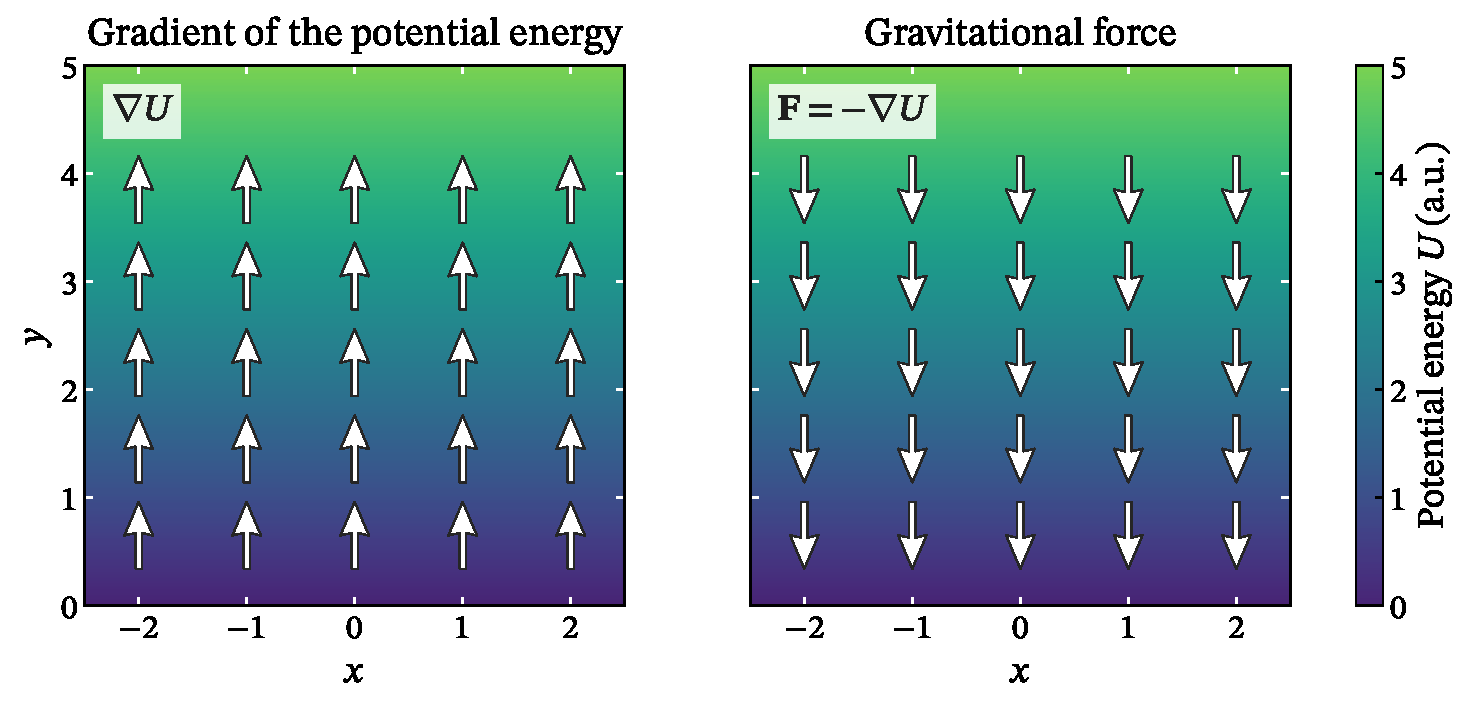
\includegraphics[width=0.8\textwidth]{scripts/gravitational_gradient.pdf}
	\caption{The potential-energy gradient and the corresponding gravitational
		force in a uniform gravitational field.}
	\label{fig:gravitational-potential-gradient}
\end{figure}

The gradient, as shown in \cref{fig:gravitational-potential-gradient},
points upward, in the direction in which the potential energy increases most
rapidly. The gravitational force is
\[
	F = - \nabla U = (0,-mg,0),
\]
and therefore points downward, toward the decreasing potential energy.

\newpage\newpage
\subsection{The potential}

The potential energy is not an exclusive property of the field; it depends also on the
body used to probe it.

Near the surface of the Earth, for instance,
\[
	U(y) = mgy.
\]
At the same height \(y\), two bodies of different mass have different potential energies.
This does not mean that they experience different gravitational fields: the field is
the same, and what changes is the amount of matter on which it acts.

We can therefore separate the two contributions by dividing the potential energy
by the property of the body that fixes the strength of the interaction; in the
gravitational case, its mass:
\[
	\phi(r) = \frac{U(r)}{m}.
\]
The function \(\phi(r)\) is called the gravitational potential, and consequently,
in the gravitational case,
\[
	U(r) = m \phi(r).
\]
Here \(\phi\) carries the information about the field, while \(m\) the information
about the probe. Taking the gradient
\[
	F = - \nabla U = -m \nabla \phi \implies g \equiv \frac{F}{m} = - \nabla \phi,
\]
so the potential stands to the field exactly as the potential energy stands to the
force.

The same construction applies to any conservative interaction, once the coupling is
factored out. For the electrostatic force the role of the mass is played by the
electric charge \(q\):
\[
	V(r) = \frac{U(r)}{q}, \qquad E = - \nabla V,
\]
where \(V\) is the electric potential.


Notice now that \(U\) never enters the physics by itself: it enters only
through its gradient. This has an immediate consequence. If \(c\) is any constant
and we replace
\[
	U(r) \mapsto U(r) + c,
\]
then, since differentiation annihilates constants, \(\nabla c = 0\) and
\[
	\nabla (U + c) = \nabla U.
\]
The force is unchanged, and so is every trajectory it produces. The same holds for
the potential, \(\phi \mapsto \phi + c/m\). Two potential energies that differ by a
constant are therefore physically indistinguishable: they are not two competing
descriptions of which one is correct, but two labels for the same identical physical
situation.
